\documentclass[12pt]{article}

%opening
\title{Unimathematik für Informatikstudiengänge \\ Zusammenfassung}
\author{Konstantin Lukas}
\renewcommand{\contentsname}{Inhaltsverzeichnis}
\usepackage{xstring}
\usepackage{catchfile}

\newcommand{\monthword}[1]{\ifcase#1\or Januar\or Februar\or März\or April\or
	Mai\or Juni\or Juli\or August\or
	September\or Oktober\or November\or Dezember\fi}
\date{Fassung vom \the\day . \monthword{\month} \the\year}
\usepackage{amsmath,amsfonts,amssymb,amsthm}
\usepackage{braket}
\usepackage[margin=2cm]{geometry}
\usepackage{bbold}
\usepackage{pgffor,listofitems}
\usepackage{tocloft}
\usepackage{etoc}
\usepackage{blindtext}
\usepackage{tikz}
\usepackage{array}
\usepackage[most]{tcolorbox}
\usepackage[hidelinks]{hyperref}
\usepackage{pgfplots}
\usepackage{tocloft}
\usepackage{polynom}
\usepackage{tkz-euclide}
\definecolor{gridgray}{HTML}{AAAAAA}
\renewcommand{\cftsecleader}{\cftdotfill{\cftdotsep}}
\DeclareRobustCommand{\bigfrac}[3][5pt]{%
	\frac{\hspace{#1}#2\hspace{#1}}{\hspace{#1}#3\hspace{#1}}}
\newcommand{\highlight}[2]{\textcolor{blue}{\hyperref[#1]{#2}} (S. \pageref{#1})}
\newcommand{\getcolor}[1]{\ifcase#1\or blue\or red\or teal\or violet\or
	magenta\or orange\or purple\or brown\fi}
\newcommand{\makeplot}[8]{
	\readlist\xlimits{#4}
	\def\xlower{\xlimits[1]}
	\def\xupper{\xlimits[2]}
	\readlist\ylimits{#5}
	\def\ylower{\ylimits[1]}
	\def\yupper{\ylimits[2]}
	\readlist\dimensions{#8}
	\def\width{\dimensions[1]}
	\def\height{\dimensions[2]}
	\begin{center}
		\begin{tikzpicture}
		\begin{axis}[
		domain=\xlower:\xupper,
		width=\width,
		height=\height,
		restrict y to domain=#6,
		xmin=\xlower, xmax=\xupper,
		ymin=\ylower, ymax=\yupper,
		samples=#7,
		axis y line=center,
		axis x line=middle,
		ticklabel style={fill=white},
		minor tick num=2,
		grid=both,
		grid style={line width=.1pt, draw=gridgray!10},
		major grid style={line width=.2pt,draw=gridgray!50}
		]
		\foreach \graph [count=\i] in {#1} {
			\edef\temp{\noexpand\addplot+[mark=none, color=\getcolor{\i}, solid] {\graph};}
			\temp
		}
		
		
		\end{axis}
		\readlist\pos{#3}
		\foreach \label [count=\i] in {#2} {
			\node [color=\getcolor{\i}] at (\pos[\i]) {\label};
		}
		
		\end{tikzpicture}
	\end{center}
}

\begin{document}
\maketitle
\tableofcontents
\pagebreak
\etocsettocstyle{\noindent\rule{\linewidth}{.4pt}}

\section{Mengen}
	\subsection{Vereinigung}
		\begin{flalign*}
			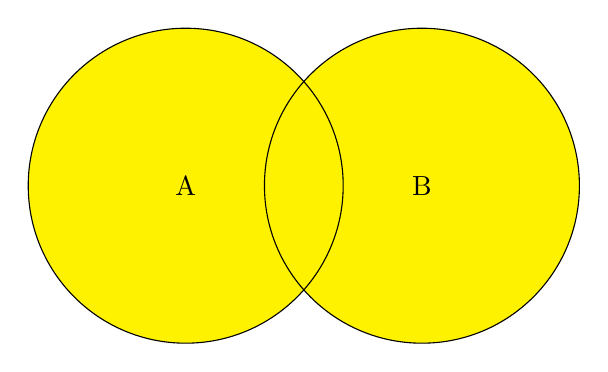
\begin{tikzpicture}
			\fill[yellow] (3,0) circle (2cm);
			\fill[yellow] (0,0) circle (2cm);
			\draw (0,0) circle (2cm);
			\draw (3,0) circle (2cm);
			\draw (0,0) node {A};
			\draw (3,0) node {B};
			\end{tikzpicture}&&
		\end{flalign*}
		\begin{flalign*}
			A \cup B := \{x \mid x \in A \: oder \: x \in B\}&&
		\end{flalign*}
	\subsection{Durchschnitt}
		\begin{flalign*}
			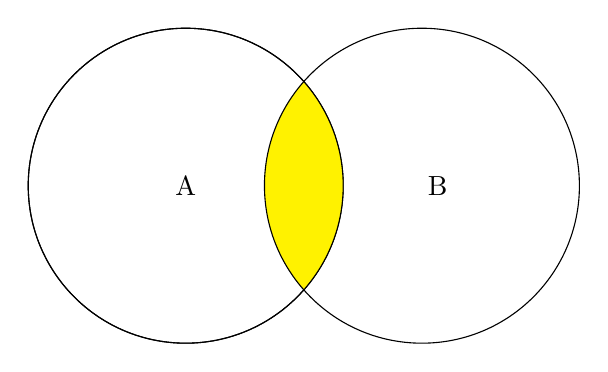
\begin{tikzpicture}
			\begin{scope}
				\draw [clip](0,0) circle (2cm);
				\fill[yellow] (3,0) circle (2cm);
			\end{scope}
			\draw (0,0) circle (2cm);
			\draw (3,0) circle (2cm);
			\draw (0,0) node {A};
			\draw (3.2,0) node {B};
			\end{tikzpicture}&&
		\end{flalign*}
		\begin{flalign*}
			A \cap B := \{x \mid x \in A \: und \: x \in B\}&&
		\end{flalign*}
	\subsection{Differenz}
		\begin{flalign*}
			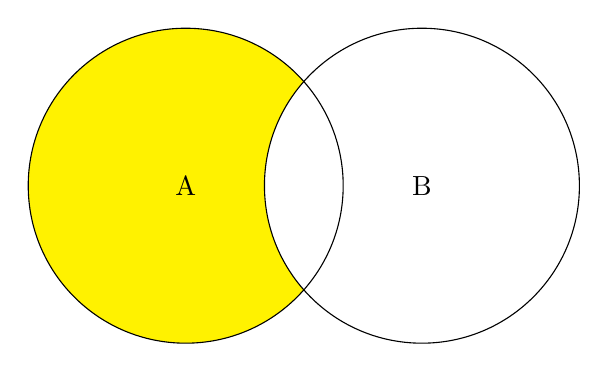
\begin{tikzpicture}
			\begin{scope}
				\fill[yellow] (0,0) circle (2cm);
				\clip (3,0) circle(2cm);
				\fill[white] (3,0) circle (2cm);
			\end{scope}
			\draw (0,0) circle (2cm);
			\draw (3,0) circle (2cm);
			\draw (0,0) node {A};
			\draw (3,0) node {B};
			\end{tikzpicture}&&
		\end{flalign*}
		\begin{flalign*}
			A \setminus B := \{x \mid x \in A \: und \: x \notin B\}&&
		\end{flalign*}
	\subsection{Symmetrische Differenz}
		\begin{flalign*}
			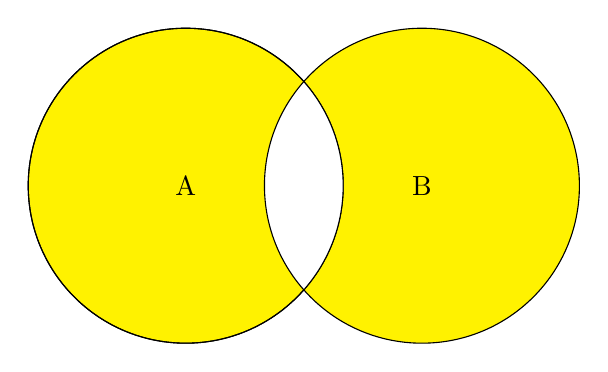
\begin{tikzpicture}
				\fill[yellow] (0,0) circle (2cm);
				\fill[yellow] (3,0) circle (2cm);
				\begin{scope}
					\draw [clip](0,0) circle (2cm);
					\fill[white] (3,0) circle (2cm);
				\end{scope}
				\draw (0,0) circle (2cm);
				\draw (3,0) circle (2cm);
				\draw (0,0) node {A};
				\draw (3,0) node {B};
				\end{tikzpicture}&&
			\end{flalign*}
		\begin{flalign*}
			A \triangle B := \{ x \mid (x \in A) \: \veebar \: ( x \in B ) \}&&
			A \triangle B := \{ x \mid (x \in A) \: \nleftrightarrow \: ( x \in B ) \}&&
		\end{flalign*}
	\subsection{Definierte Zahlenmengen}
	Natürliche Zahlen
		\begin{flalign*}
			\mathbb{N} = \{ 1; 2; 3; ... \}&&
		\end{flalign*}\newline
	Menge der Natürliche Zahlen
		\begin{flalign*}
			\mathbb{N}_0 = \{ 0; 1; 2; 3; ... \}&&
		\end{flalign*}\newline
	Ganze Zahlen
		\begin{flalign*}
			\mathbb{Z} = \{ ... ; -2; -1; 0; 1; 2; 3; ... \}&&
		\end{flalign*}\newline
	Rationale Zahlen
		\begin{flalign*}
			\mathbb{Q} = \left\{ \frac{p}{q} \mid p, q \in \mathbb{Z}, q \neq 0 \right\}&&
		\end{flalign*}\newline
		Reelle Zahlen\newline
		Die reellen Zahlen umfassen die rationalen Zahlen und die irrationalen Zahlen.\newline\newline
		Irrationale Zahlen
		\begin{flalign*}
			\mathbb{R} \setminus \mathbb{Q}&&
		\end{flalign*}
\section{Elementare Rechengesetze, -verfahren und -notationen}
	\subsection{Brüche dividieren}
		Um zwei Brüche zu dividieren bildet man den Kehrwert vom Divisor und multipliziert diesen mit dem Dividend.
		\begin{flalign*}
		\frac{p_1}{q_1} : \frac{p_2}{q_2} = \frac{p_1}{q_1} \cdot \frac{q_2}{p_2}&&
		\end{flalign*}
		\begin{flalign*}
		\bigfrac {\frac{p_1}{q_1}}  {\frac{p_2}{q_2}} = \frac{p_1}{q_1} \cdot \frac{q_2}{p_2}&&
		\end{flalign*}
	\subsection{Lösungsmenge}
		Beispiel 1 ($x^2=-1$):\newline
		$\mathbb{L} = \emptyset$ \newline\newline
		Beispiel 2 ($x^2 = 4$):\newline
		$\mathbb{L} = \{-2;2\}$\newline\newline
		Beispiel 3 ($sin(x) = 0$):\newline
		$\mathbb{L} = \{...;-2\pi;-\pi;0;\pi;2\pi; ...\}$\newline\newline
		Beispiel 4 ($x^2 + y = 5$):\newline
		$\mathbb{L} = \{(x_0;y_0)\in\mathbb{R}^2\mid x^2_0 + y_0 = 5\} = \{(x_0;5-x^2_0) \mid x_0\in\mathbb{R}^2\}$\newline\newline
		In diesem Fall ist die Lösungsmenge die Funktion $y=5-x^2$.\newline
		\makeplot{{5-x^2}}{{$f(x)=5-x^2$}}{{11,3.3}}{-10,10}{-10,10}{-30:30}{330}{17cm,7cm}
	\subsection{Normalform}
		Eine Gleichung in der Form $ax^2+bx+c=0$ mit $a\neq0$ und $b,c\in \mathbb{R}$, heißt quadratisch. Spezial bezeichnet man $x^2+px+q=0$ mir $p,q\in \mathbb{R}$, als quadratische Gleichung in Normalform.\newline\newline
		Man kann eine quadratische Gleichung in die Normalform überführen, indem man durch $a$ teilt: $x^2+\frac{b}{a}x+\frac{c}{a}=0$.
		\subsubsection{p-q-Formel}
		\label{subsubsec:pqformel}
		\begin{tcolorbox}[boxsep=0pt,top=.75cm,left=1cm,right=1cm, bottom=.5cm,arc=0pt,auto outer arc,colback=white,colframe=black, enlarge top by=.25cm, enlarge bottom by=.25cm]
			Um die Nullstellen einer quadratischen Gleichung in der Normalform zu finden, kann man die p-q-Formel benutzen: $x_{\pm}=-\frac{p}{2}\pm\sqrt{\left(\frac{p}{2}\right)^2-q}$.
		\end{tcolorbox}
		\noindent$D=\left(\frac{p}{2}\right)^2-q$ ist die Diskriminante. Sie gibt Aufschluss über die Lösungsmenge.
		\begin{flalign*}
		&D>0\Rightarrow Es\;gibt\;zwei\;Lsg.\\
		&D=0\Rightarrow Es\;gibt\;eine\;Lsg.\\
		&D<0\Rightarrow Es\;gibt\;keine\;Lsg.&&
		\end{flalign*}
	\subsection{Intervalle}
		\label{subsec:intervalle}
		\subsubsection{Abgeschlossene Intervalle}
		$[a;b] := \{ x \in \mathbb{R} \mid a \le x \le b \}$
		\subsubsection{Offene Intervalle}
		$(a;b) = \: ]a;b[ \: := \{ x \in \mathbb{R} \mid a < x < b \}$
		\subsubsection{Halboffene Intervalle}
		Rechtsoffen \newline
		$[a;b) = \: [a;b[ \: :=  \{ x \in \mathbb{R} \mid a \le x < b \}$ \newline\newline
		Linksoffen \newline
		$(a;b] = \: ]a;b] \: :=  \{ x \in \mathbb{R} \mid a < x \le b \}$
	\subsection{Beträge}
		\begin{flalign*}
		\vert a \vert = \left\{ a \atop -a \right. \;\;&
		a \ge 0 \atop a < 0 &
		\end{flalign*}
		\begin{flalign*}
		\vert -a \vert = \vert a \vert&&
		\end{flalign*}
	\subsection{Binomische Formeln}
	\label{sec:binomischeformeln}
	$(a+b)^2 = a^2 + 2ab + b^2$ \newline\newline
	$(a-b)^2 = a^2 - 2ab + b^2$ \newline\newline
	$(a+b)(a-b) = a^2 - b^2$
	\subsection{Euklidischer Algorithmus}
		Der euklidische Algorithmus findet den größten gemeinsamen Teiler zweier Zahlen. Das eignet sich ausgezeichnet dazu, Brüche zu kürzen. Der vorletzte Rest bevor $R = 0$ eintritt, ist das Ergebnis.
		\begin{flalign*}
		& 2160 : 2592 = 0 \;\;\; R = 2160 \\
		& 2592 : 2160 = 1 \;\;\; R = 432 \\
		& 2160 : 432 = 5 \;\;\; R = 0 &&
		\end{flalign*}
		\begin{flalign*}
		\frac{2592}{2160} = \frac{6 \cdot 432}{5 \cdot 432} = \frac{6}{5}&&
		\end{flalign*}
	\subsection{Potenzgesetze}
	\label{subsec:potenzgesetze}
		\begin{tcolorbox}[boxsep=0pt,top=.35cm,left=1cm,right=1cm, bottom=.75cm,arc=0pt,auto outer arc,colback=white,colframe=black, enlarge top by=.25cm, enlarge bottom by=.25cm]
			\begin{flalign*}
				& a^k \cdot a^m = a^{k+m} \\\\
				& \cfrac{b^k}{b^m} = b^{k-m} \\\\
				& a^k \cdot b^k = (a \cdot b)^k \\\\
				& \cfrac{a^k}{b^k} = \left( \frac{a}{b} \right)^k \\\\
				& (a^k)^m = a^{k \cdot m} && 
			\end{flalign*}
		\end{tcolorbox}
		\noindent Für $a>0$ und jede rationale Zahl $\frac{p}{q}$ (mit $p,q \in \mathbb{Z}$ und $q>0$) ist
		\begin{flalign*}
		a^{\frac{p}{q}} = \sqrt[q]{a^p} = (\sqrt[q]{a})^p && 
		\end{flalign*}
		Beispiel: Bestimmen Sie $m$ und $n$ so, dass gilt: $(9x^7)^2 = mx^n$
		\begin{flalign*}
			(9x^7)^2 = mx^n \\
			81x^{14} = mx^n &&
		\end{flalign*}
		$m = 81$ und $n = 14$
	\subsection{Wurzelgesetze}
		\begin{tcolorbox}[boxsep=0pt,top=.75cm,left=1cm,right=1cm, bottom=.7cm,arc=0pt,auto outer arc,colback=white,colframe=black, enlarge top by=.25cm, enlarge bottom by=.25cm]
			Für $a,b,c \in \mathbb{R}$ mit $a,b \ge 0, c > 0$ und $m, n \in \mathbb{N}$ gilt
			\begin{flalign*}
				& \sqrt[n]{ab} = \sqrt[n]{a} \cdot \sqrt[n]{b} \\\\
				& \sqrt[n]{\frac{a}{c}} = \frac{\sqrt[n]{a}}{\sqrt[n]{c}} \\\\
				& \sqrt[n]{\sqrt[m]{a}} = \sqrt[n \cdot m]{a} && 
			\end{flalign*}
		\end{tcolorbox}
		\noindent Beispiel 1: Nach der dritten Binomischen Formel gilt für $a,b > 0, a \neq b$:
		\begin{flalign*}
		& \cfrac{1}{\sqrt{a}+\sqrt{b}} & \mid \cdot (\sqrt{a}-\sqrt{b}) &&&&&&&&&&&& \\
		= & \cfrac{\sqrt{a}-\sqrt{b}}{(\sqrt{a}+\sqrt{b})(\sqrt{a}-\sqrt{b})} \\ 
		= & \cfrac{\sqrt{a}-\sqrt{b}}{\sqrt{a}^2-\sqrt{b}^2} \\ 
		= & \cfrac{\sqrt{a}-\sqrt{b}}{a-b} &&
		\end{flalign*}
		\hrulefill\newline\newline
		Beispiel 2:
		\begin{flalign*}
		& \frac{\sqrt{(1+a^2) \cdot (a-b)^2}}{\sqrt[4]{16(1+a^2)^2}} \\
		= & \sqrt{\frac{(1+a)^2 \cdot (a-b)^2}{\sqrt{16(1+a^2)^2}}} \\ 
		= & \sqrt{\frac{(1+a)^2 \cdot (a-b)^2}{4(1+a)^2}} \\ 
		= & \frac{1}{2}\sqrt{(a-b)^2} \\ 
		= & \frac{\mid a-b \mid}{2} &&
		\end{flalign*}
		\subsubsection{Wurzeltherme vereinfachen (Beispiele)}
			\begin{flalign*}
				\sqrt{2}+\dfrac{2}{2\sqrt{2}+3} & = \dfrac{}{}\sqrt{2}+\dfrac{ 2\cdot ( 2\sqrt{2}-] ) }{\left( 2\sqrt{2}+3\right) \left( 2\sqrt{2}-3\right) } \\
				& = \sqrt{2}+\dfrac{4\sqrt{2}-6}{\left( 2\sqrt{2}\right) ^{2}-3^{2}} \\
				& = \sqrt{2}+\dfrac{4\sqrt{2}-6}{-1} \\
				& = \sqrt{2}-4\sqrt{2}+6 \\
				& = 6-3\sqrt{2} &&
			\end{flalign*}
			\hrulefill
			\begin{flalign*}
			\dfrac{1}{\sqrt{1+x^{2}}-1}-\dfrac{1}{\sqrt{1+x^{2}}+1} & = \dfrac{\sqrt{1+x^{2}}+1}{\left( \sqrt{1+x^{2}}-1\right) \cdot \left( \sqrt{1+x^{2}}+1\right) } - \dfrac{\sqrt{1+x^{2}}-1}{\left( \sqrt{1+x^{2}}+1\right) \cdot \left( \sqrt{1+x^{2}}-1\right) } \\
			& = \dfrac{\left( \sqrt{1+x^{2}}+1\right) -\left( \sqrt{1+x^{2}}-1\right) }{1+x^{2}-1} \\
			& = \frac{2}{x^2} &&
			\end{flalign*}
			\hrulefill\newline\newline
			Beispiel 3: Bestimmen Sie $x$ und $y$, sodass $\frac{x}{y}$ vollständig gekürzt ist.
			\begin{flalign*}
				\dfrac{2\cdot 2^{\frac{5}{2}}}{2^{\frac{1}{4}}}=2^{\frac{x}{y}} \\
				2 \cdot \dfrac{2^{\frac{5}{2}}}{2^{\frac{1}{4}}}=2^{\frac{x}{y}} \\
				2 \cdot 2^{\frac{5}{2}-\frac{1}{4}} = 2^{\frac{x}{y}} \\
				2 \cdot 2^{\frac{9}{4}} = 2^{\frac{x}{y}} \\
				2^{\frac{13}{4}} = 2^{\frac{x}{y}} &&
			\end{flalign*}
			Damit gilt $x = 13$ und $y = 4$.
	\subsection{Logarithmusgesetze}
	\label{subsec:logarithmusgesetze}
		\begin{tcolorbox}[boxsep=0pt,top=1cm,left=1cm,right=1cm, bottom=1cm,arc=0pt,auto outer arc,colback=white,colframe=black, enlarge top by=.25cm, enlarge bottom by=.25cm]
			Die Logarithmusrechnung dient dazu das $x$ im Term $b^x=a$ zu bestimmen. Es ist damit quasi das Gegenstück zur Potenzrechnung. Rechnen wir z.~B. $9^3$, kommen wir auf $729$. Umgekehrt können wir jetzt aber auch $log_{9}729$ rechnen und kommen auf $3$. Es gibt außerdem die speziellen Notationen $ln$ und $lg$, die jeweils \textit{natürlicher Logarithmus} und \textit{dekadischer Logarithmus} genannt werden.
			\begin{flalign*}
				ln(b):=log_e(b)&&
			\end{flalign*}
			\begin{flalign*}
				lg(b):=log_{10}(b)&&
			\end{flalign*}
			\begin{flalign*}
				log_b(b)=1&&
			\end{flalign*}
			\begin{flalign*}
				log_b(1)=0&&
			\end{flalign*}
			\begin{flalign*}
				log_b(u\cdot v)=log_b(u)+log_b(v)&&
			\end{flalign*}
			\begin{flalign*}
				log_b\left(\frac{u}{v}\right)=log_b(u)-log_b(v)&&
			\end{flalign*}
			\begin{flalign*}
				log_b(u^v)=v\cdot log_b(u)&&
			\end{flalign*}
			\begin{flalign*}
				log_b(\sqrt[u]{v})=\frac{log_b(v)}{u}&&
			\end{flalign*}
			\begin{flalign*}
				log_a(v)=\frac{log_b(v)}{log_b(a)}&&
			\end{flalign*}
		\end{tcolorbox}
\section{Vereinfachungen zum Lösen von Gleichungen}
	\subsection{Quadratische Ergänzung}
		\begin{tcolorbox}[boxsep=0pt,top=.75cm,left=1cm,right=1cm, bottom=.65cm,arc=0pt,auto outer arc,colback=white,colframe=black, enlarge top by=.25cm, enlarge bottom by=.25cm]
			Die äquivalente Umformung der quadratischen Gleichung in Normalform $x^2+px+q=0$ in $\left(x+\frac{p}{2}\right)^2=-q+\left(\frac{p}{2}\right)^2$ wird als quadratische Ergänzung bezeichnet. In anderen Worten fügt man den Term $+\left(\frac{p}{2}\right)^2-\left(\frac{p}{2}\right)^2$ hinzu.
		\end{tcolorbox}
		\noindent Beispiel:
			\begin{flalign*}
		x^2+8x+7 &= 0\\
		x^2+8x+\left(\frac{8}{2}\right)^2+\left(\frac{8}{2}\right)^2+7 &= 0\\
		x^2+8x+4^2+4^2+7 &= 0\\
		(x+4)^2+4^2+7 &= 0\\
		(x+4)^2-9 &= 0\;\;\;\;\;\;\;\;\;\mid+9\\
		(x+4)^2 &= 9\;\;\;\;\;\;\;\;\;\mid\sqrt{\ }\\
		x&=\pm\sqrt{9}-4\\
		\mathbb{L}&=\{-1;-7\}&&
		\end{flalign*}
	\subsection{Faktorisieren}
		Um die Nullstellen eines Terms zu finden, bietet es sich an, ihn als Produkt einfacher Terme zu schreiben, denn ist ein Faktor $0$, ist das Produkt ebenfalls $0$. Den Term in so eine Form zu überführen, nennt sich Faktorisieren.
		\subsubsection{Faktorisierung durch Ausklammern}
		\label{subsubsec:ausklammern}
			Beispiel:
			\begin{flalign*}
				x^4+2x^3+3x^2 &= 0\\
				x^2(x^2+2x+3) &= 0\\
				x^2 &= 0\;oder\;(x^2+2x+3) = 0\\
				\mathbb{L} &= \{0\}&&
			\end{flalign*}
			Für $x^2+2x+3 = 0$ existiert keine reelle Lösung $\Rightarrow$ \highlight{subsubsec:pqformel}{p-q-Formel}.
		\subsubsection{Faktorisierung mit binomischen Formeln}
			Beispiel:
			\begin{flalign*}
			9x^2+30x+25& = 0\\
			(3x+5)^2& = 0\\
			3x+5&=0\;\;\;\;\;\;\;\;\;\mid-5\\
			3x&=-5\;\;\;\;\;\;\;\;\;\mid:3\\
			x&=-\frac{5}{3}\\
			\mathbb{L}&=\left\{-\frac{5}{3}\right\}&&
			\end{flalign*}
		\subsubsection{Faktorisierung mit dem Satz von Viëta}
			\begin{tcolorbox}[boxsep=0pt,top=.75cm,left=1cm,right=1cm, bottom=.75cm,arc=0pt,auto outer arc,colback=white,colframe=black, enlarge top by=.25cm, enlarge bottom by=.25cm]
			Der Satz von Viëta besagt, dass $x^2+px+q=(x-x_1)\cdot(x-x_2)$ ist. $p$ und $q$ lassen sich auf die Nullstellen zurückführen: $x_1+x_2=-p$ und $x_1\cdot x_2 = q$.
			\end{tcolorbox}
			\noindent Daraus lässt sich $x_2=\frac{q}{x_1}$ ableiten. Wenn man also durch Raten eine Nullstelle findet, kann man so die andere Nullstelle auch ganz einfach finden.\newline\newline
			Beispiel (eine Nullstelle ist $1$, die andere ergibt sich als $\sqrt{2} = \frac{\sqrt{2}}{1}$):
			\begin{flalign*}
				x^2+(\sqrt{2}-1)x-\sqrt{2}&=0\\
				(x-1)\cdot (x+\sqrt{2})&=0\\
				\mathbb{L}=\{1;-\sqrt{2}\}&&
			\end{flalign*}
	\subsection{Substitution}
	\label{subsec:substitution}
		Substitution erlaubt es uns manchmal Gleichungen zu vereinfachen, um leichter mit ihnen rechnen zu können.\newline\newline
		Beispiel: $x^8-15x^4-16=0$\newline
		Hier bietet es sich an $x^4$ durch $u$ zu ersetzen.
		\begin{flalign*}
		u^2-15u-16&=0\\
		u_{\pm}&=\frac{15}{2}\pm\sqrt{\left(\frac{-15}{2}\right)^2+6}&&
		\end{flalign*}
		Diesen Term wiederum können wir ganz einfach mit der \highlight{subsubsec:pqformel}{p-q-Formel} lösen. Dabei erhalten wir $u_+=16$ und $u_-=-1$. Um unsere endgültige Lösungsmenge zu bekommen, müssen wir noch resubstituieren.
		\begin{flalign*}
		x^4&=u_+=16\\
		x_1&=2\\
		x_2&=-2&&
		\end{flalign*}
		Da es kein $x$ gibt, das $x^4=-1$ erfüllt, haben wir bereits unsere komplette Lösungsmenge:\newline\newline$\mathbb{L}=\{-2;2\}$.
\section{Ungleichungen}
	\subsection{Rechenregeln}
	\label{subsec:unglrechrgl}
		Wenn man ein Ungleichung mit einer negativen Zahl multipliziert oder durch diese teilt, muss das Vergleichszeichen umgekehrt werden.
		\begin{tcolorbox}[boxsep=0pt,top=.75cm,left=1cm,right=1cm, bottom=.65cm,arc=0pt,auto outer arc,colback=white,colframe=black, enlarge top by=.25cm, enlarge bottom by=.25cm]
			Für $c<0$ gilt:
			\begin{flalign*}
				&a<b\iff c\cdot  a>c\cdot b\\
				&a<b\iff \frac{a}{c}>\frac{b}{c} &&
			\end{flalign*}
		\end{tcolorbox}
	\subsection{Quadratische Ungleichungen}
		Um die Lösungsmenge einer quadratischen Ungleichung zu finden, formt man die Ungleichung zunächst so um, dass auf einer Seite $0$ steht. Auf der anderen Seite hat man dann optimalerweise eine quadratische Funktion. Schauen wir uns mal das Beispiel $x^2>2x+7$ an.
		\makeplot{{x^2-2*x-7}}{{$f(x)=x^2-2x-7$}}{{5,1}}{-10,10}{-10,10}{-30:30}{330}{17cm,7cm}
		Wir stellen also zunächst um und erhalten $x^2-2x-7>0$. Daraus ergibt sich auch die Funktion oben. An der Grafik erkennt man sehr gut, was wir eigentlich suchen. Denn unsere Lösungsmenge sind alle $x$, für die $f(x)$ größer als $0$ ist. Und wie kriegen wir das raus? Indem wir die Nullstellen berechnen. Das Intervall von Unendlich bis zur linken Nullstelle ist ein Teil unserer Lösung und der andere ist das Intervall von der rechten Nullstelle bis unendlich. Dabei muss man stets verschiedene Fälle beachten. Für eine nach unten geöffnete Funktion ($-x^2$) suchen wir den Bereich zwischen den Nullstellen. Für eine Funktion oberhalb der $x$-Achse, die keine Nullstellen hat, sind alle reellen Zahlen unsere Lösungsmenge, wohingegen eine Funktion ohne Nullstellen unterhalb der $x$-Achse eine leere Lösungsmenge liefern würde. Eine Funktion mit genau einer Nullstelle liefert hingegen eine Lösungsmenge aller reellen Zahlen außer der Nullstelle. Es gibt je nach Art der Funktion und Vergleichszeichen in unserer Ungleichung viele unterschiedliche Szenarien, weshalb es immer ratsam ist eine Skizze anzufertigen. Für das Beispiel oben können wir die \highlight{subsubsec:pqformel}{p-q-Formel} verwenden, um die Nullstellen zu berechnen.
		\begin{flalign*}
		x_{\pm}&=-\frac{-2}{2}\pm \sqrt{\left(\frac{-2}{2}\right)^2+7}\\
		x_1&=1-2\sqrt{2}\\
		x_2&=1+2\sqrt{2}&&
		\end{flalign*}
		Jetzt, wo wir die Nullstellen haben, ist es nicht schwer die Lösungsmenge anzugeben. Dabei sollte man darauf achten, dass man abgeschlossene und offene \highlight{subsec:intervalle}{Intervalle} nicht verwechselt.
		\begin{flalign*}
			\mathbb{L}=\mathbb{R}\setminus \left[1-2\sqrt{2};1+2\sqrt{2}\right]=\left(-\infty;1-2\sqrt{2}\right)\cup\left(1+2\sqrt{2}\right)&&
		\end{flalign*}
	\subsection{Ungleichungen mit Beträgen}
		Das Vorgehen bei Betragsungleichungen ist im Grunde genommen dasselbe Prinzip, wie bei den quadratischen. Schauen wir uns das Beispiel $\vert x \vert -3 < 0$ an.
		\makeplot{{abs(x)-3}}{{$f(x)=\vert x \vert -3$}}{{5,1.75}}{-10,10}{-10,10}{-30:30}{330}{17cm,7cm}
		Wir erkennen die Nullstellen in dem Fall sehr leicht. Das sind $-3$ und $3$. Erkennt man das nicht sofort, muss man eine \highlight{subsec:betragsfunktionen}{Fallunterscheidung} durchführen. Jetzt können wir aber erst mal unsere Lösungsmenge definieren, denn wir wissen, dass wir alle $x$ suchen für die $f(x)<0$ gilt.
		\begin{flalign*}
		\mathbb{L}=(-3;3)&&
		\end{flalign*}
		Hinweis: Wäre unsere Ausgangsungleichung $\vert x \vert -3 \le 0$, sehe unsere Lösungsmenge jetzt so aus:
		\begin{flalign*}
		\mathbb{L}=[-3;3]&&
		\end{flalign*}
	\subsection{Ungleichungen mit Variable im Nenner – Teil I}
		Aus den vorherigen Erklärungen kann man sich herleiten, wie man das macht. Deshalb ist hier nur noch mal ein erklärendes Beispiel: $2\le \frac{14}{\vert 2x+5\vert}$.
		\makeplot{{(14/abs(2*x+5))-2}}{{$f(x)=\dfrac{14}{\vert 2x+5\vert}-2$}}{{10,3.5}}{-10,10}{-10,10}{-30:30}{200}{17cm,7cm}
		Wichtig ist, dass wir zunächst alle $x$ ausschließen, für die im Nenner $0$ rauskommt. In diesem Fall ist dass $-\frac{5}{2}$.
		\begin{flalign*}
			2&\le \frac{14}{\vert 2x+5\vert}\\
			2\vert 2x+5\vert&\le 14\\
			\vert 2x+5\vert&\le 7&&
		\end{flalign*}
		Fall 1: $2x+5>0$
		\begin{flalign*}
		2x+5&\le 7\\
		2x&\le 2\\
		x&\le 1&&
		\end{flalign*}
		Fall 2: $2x+5<0$
		\begin{flalign*}
		-2x-5&\le 7\\
		-2x&\le 12\\
		x&\ge -6&&
		\end{flalign*}
		\begin{flalign*}
		\mathbb{L}=\left[-6;-\frac{5}{2}\right)\cup\left(-\frac{5}{2};1\right]&&
		\end{flalign*}
	\subsection{Ungleichungen mit Variable im Nenner – Teil II}
		Wenn wir uns an die \highlight{subsec:unglrechrgl}{Rechenregeln} für Ungleichungen erinnern, könnte man sich fragen, was passiert, wenn der Nenner mit einer Variable sowohl positiv als auch negativ sein kann. Denn wenn wir mit einer negativen Zahl multiplizieren, müssten wir das Vorzeichen umkehren. Hier muss man wieder verschiedene Fälle unterscheiden.\newline\newline
		Beispiel: $\frac{1}{x-2}\le-x$
		\makeplot{{(1/(x-2))+x}}{{$f(x)=\dfrac{1}{x-2}+x$}}{{11.1,0.65}}{-10,10}{-10,10}{-20:20}{350}{17cm,7cm}
		Der Fall $x=2$ ist aufgrund des $x$ im Nenner wieder auszuschließen.
		Fall 1: $x>2$
		\begin{flalign*}
			\frac{1}{x-2}&\le-x\\
			1&\le -x(x-2)\\
			1&\le -x^2+2x\\
			x^2-2x+1&\le 0\\
			(x-1)^2&\le 0&&
		\end{flalign*}
		Dieser Fall gilt für $x=1$. Das widerspricht allerdings der Bedingung $x>2$ und das Ergebnis ist entsprechend nicht Teil unserer Lösungsmenge.\newline\newline
		Fall 2: $x<2$
		\begin{flalign*}
			\frac{1}{x-2}&\le-x\\
			1&\ge -x(x-2)\\
			1&\ge -x^2+2x\\
			x^2-2x+1&\ge 0\\
			(x-1)^2&\ge 0&&
		\end{flalign*}
		Dieser Fall ist für alle $x$ erfüllt, daher gehören alle $x<2$ zur Lösungsmenge.
		\begin{flalign*}
			\mathbb{L}=(-\infty;2)&&
		\end{flalign*}\hrulefill\newline\newline
		Beispiel: $\frac{1}{x-9}\le8$
		\makeplot{{(1/(x-9))-8}}{{$f(x)=\dfrac{1}{x-9}-8$}}{{11,1.6}}{-2,16}{-20,5}{-30:60}{330}{17cm,7cm}
		Fall 1: $x>9$
		\begin{flalign*}
			\frac{1}{x-9}&\le 8\\
			1&\le 8x-72\\
			8x&\ge 73\\
			x&\ge \frac{73}{8}&&
		\end{flalign*}
		Fall 2: $x<9$
		\begin{flalign*}
			\frac{1}{x-9}&\le 8\\
			1&\ge 8x-72\\
			8x&\le 73\\
			x&\le \frac{73}{8}&&
		\end{flalign*}
		\begin{flalign*}
			\mathbb{L}=(-\infty;9)\cup \left[\frac{73}{8};\infty\right)&&
		\end{flalign*}
	\section{Lineare Gleichungssysteme}
		Ein Gleichungssystem ist eine Sammlung an Gleichungen, für die man eine gemeinsame Lösung sucht. Für das Beispiel unten, ist die Lösung $x=2,y=3,z=-4$ oder anders ausgedrückt $\mathbb{L}=\{(2;3;-4)\}$. Wie man darauf kommt, wird unten erklärt.
		\begin{flalign*}
			(I)&&x+2y+z&=4\\
			(II)&&x-y+ \frac{3}{2}z&=-7\\
			(III)&&-4x+2y&=-2&&&&&&&&
		\end{flalign*}
		\subsection{Einsetzungsverfahren}
			Eine Möglichkeit hat man, wenn man eine Funktion nach einer beliebigen Variable umstellt und diese dann in einer anderen Funktion einsetzt.\newline\newline
			$(III)$
			\begin{flalign*}
				-4x+2y&=-2\\
				-4x&=-2-2y\\
				x&=\frac{1}{2}+\frac{1}{2}y&&
			\end{flalign*}
			$(I)$
			\begin{flalign*}
				x+2y+z&=4\\
				\frac{1}{2}+\frac{1}{2}y+2y+z&=4\\
				\frac{1}{2}+\frac{5}{2}y+z&=4\\
				z&=3,5-\frac{5}{2}y&&
			\end{flalign*}
			$(II)$
			\begin{flalign*}
				x-y+ \frac{3}{2}z&=-7\\
				\frac{1}{2}+\frac{1}{2}y-y+ \frac{3}{2}\left(3,5-\frac{5}{2}y\right)&=-7\\
				\frac{1}{2}+\frac{1}{2}y-y+ 5,25-\frac{15}{4}y&=-7\\
				5,75-\frac{1}{2}y-\frac{15}{4}y&=-7\\
				-\frac{17}{4}y&=-\frac{51}{4}\\
				y&=3&&
			\end{flalign*}
			$(III)$
			\begin{flalign*}
				-4x+2y&=-2\\
				-4x+2\cdot 3&=-2\\
				-4x+6&=-2\\
				-4x&=-8\\
				x&=2&&
			\end{flalign*}
			$(I)$
			\begin{flalign*}
				x+2y+z&=4\\
				2+2\cdot 3+z&=4\\
				z&=-4&&
			\end{flalign*}
		\subsection{Additionsverfahren}
			Eine andere Möglichkeit ist es, eine oder mehrere Gleichungen mit einer Zahl zu multiplizieren, sodass eine Variable entfällt, wenn man zwei Gleichungen addiert.\newline\newline
			$(I)-(III)$
			\begin{flalign*}
			5x+z&=6\\
			z&=6-5x&&
			\end{flalign*}
			$(I)+2(II)$
			\begin{flalign*}
			3x+4z&=-10\\
			3x+4(6-5x)&=-10\\
			3x+24-20x&=-10\\
			-17x&=-34\\
			x&=2&&
			\end{flalign*}
			$(III)$
			\begin{flalign*}
			-4x+2y&=-2\\
			-4\cdot 2+2y&=-2\\
			-8+2y&=-2\\
			2y&=6\\
			y&=3&&
			\end{flalign*}
			$(I)$
			\begin{flalign*}
			x+2y+z&=4\\
			2+2\cdot 3+z&=4\\
			z&=-4&&
			\end{flalign*}
		Hinweis: sind zwei Gleichungen identisch, so gibt es unendlich viele Lösungsmengen und man muss nur die entsprechende Notation für die Lösungsmenge kennen.
		\begin{flalign*}
			(I)&&-4x-2y&=-14\\
			(II)&&4x+2y&=14&&&&&&&&&&&&
		\end{flalign*}
		\begin{flalign*}
			\mathbb{L}=\{(x;7-2x)\mid x \in \mathbb{R}\}&&
		\end{flalign*}
		\subsection{Gauß-Verfahren}
			Das Gauß-Verfahren ist eine bestimmte Vorgehensweise fürs Additionsverfahrens, bei dem man die Gleichungen so umformt, dass man das LGS in die Stufenform bringt und es einfach lösen kann.
			\begin{flalign*}
			(I)&&x+2y+z&=4\\
			(II)&&x-y+ \frac{3}{2}z&=-7\;\;\;\;\;\;\mid -\frac{3}{2}(I)\\
			(III)&&-4x+2y&=-2&&&&&&&&&&&&
			\end{flalign*}
			\begin{flalign*}
			(I)&&x+2y+z&=4\\
			(II)&&-\frac{1}{2}x-4y&=-13\\
			(III)&&-4x+2y&=-2\;\;\;\;\;\;\mid +\frac{1}{2}(II)&&&&&&&&&&&&
			\end{flalign*}
			\begin{flalign*}
			(I)&&x+2y+z&=4\\
			(II)&&-\frac{1}{2}x-4y&=-13\\
			(III)&&-\frac{17}{4}x&=-\frac{17}{2}&&&&&&&&&&&&
			\end{flalign*}
			$(III)$
			\begin{flalign*}
			-\frac{17}{4}x&=-\frac{17}{2}\\
			x&=2&&
			\end{flalign*}
			$(II)$
			\begin{flalign*}
			-\frac{1}{2}x-4y&=-13\\
			-1-4y&=-13\\
			-4y&=-12\\
			y&=3&&
			\end{flalign*}
			$(I)$
			\begin{flalign*}
			x+2y+z&=4\\
			2+6+z&=4\\
			z&=-4&
			\end{flalign*}
		\subsection{LGS mit Parameter}
			Kommt in einem LGS ein Parameter vor, dann muss man eine Fallunterscheidung vornehmen und den Parameter in die Lösungsmenge mit einbeziehen.
			\begin{flalign*}
			(I)&&x-2y&=0\\
			(II)&&y+\frac{1}{3}z&=-1\\
			(III)&&(a-3)y&=1&&&&&&&&&&&&
			\end{flalign*}
			Wenn $a=3$, dann kommt bei der letzten Gleichung $0=1$ raus. Dadurch können wir schon mal sagen, was die Lösungsmenge für den Fall $a=3$ ist.
			\begin{flalign*}
				\mathbb{L}=\emptyset, falls\;a=3&&
			\end{flalign*}
			Als nächstes schauen wir uns den Fall $a\neq0$ an.\newline\newline
			$(III)$
			\begin{flalign*}
				(a-3)y&=1\\
				y&=\frac{1}{a-3}&&
			\end{flalign*}
			$(II)$
			\begin{flalign*}
				\frac{1}{a-3}+\frac{1}{3}z&=-1\\
				\frac{1}{3}z&=-\frac{1}{a-3}-1\\
				z&=3\left(-\frac{1}{a-3}-1\right)\\
				z&=-\frac{3}{a-3}-\frac{3a-9}{a-3}\\
				z&=\frac{6-3a}{a-3}&&
			\end{flalign*}
			$(I)$
			\begin{flalign*}
				x-2y&=0\\
				x-2\left(\frac{1}{a-3}\right)&=0\\
				x&=\frac{2}{a-3}&&
			\end{flalign*}
			\begin{flalign*}
			\mathbb{L}=\left\{\left(\frac{2}{a-3};\frac{1}{a-3};\frac{6-3a}{a-3}\right)\right\},\;falls\;a\neq 3&&
			\end{flalign*}
	\section{Geometrie}
	\label{sec:geometrie}
		\subsection{Rechtwinklige Dreiecke}
			\begin{center}
				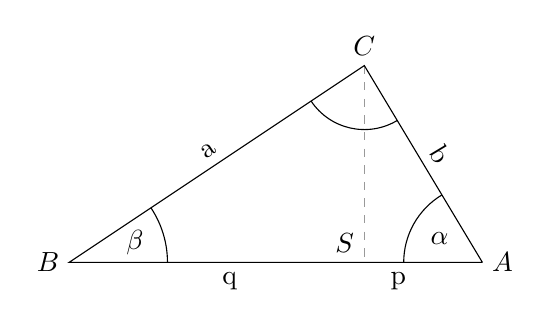
\begin{tikzpicture}[scale=1.25]%,cap=round,>=latex]
					\coordinate [label=left:$B$] (B) at (-2cm,-1.cm);
					\coordinate [label=right:$A$] (A) at (2.2cm,-1.0cm);
					\coordinate [label=above:$C$] (C) at (1cm,1.0cm);
					\coordinate [label=above:$S$] (A-|B) at (0.8cm,-1.0cm);
					\draw (A) -- node[sloped,below] {\;\;\;\;\;\;\;\;\;\;q\;\;\;\;\;\;\;\;\;\;\;\;\;\;\;\;\;\;\;\;p} (B) -- node[sloped,above] {a} (C) -- node[sloped,above] {b} (A);
					\draw[dashed, opacity=.4] (C) -- (C|-A) ;
					\tikzset{/tkzmkangle/mark=none}
					\tkzMarkAngle[size=0.65cm](B,C,A)
					
					\tkzMarkAngle[size=0.8cm](C,A,B)
					\tkzLabelAngle[pos = 0.5](C,A,B){$\alpha$}
					
					\tkzMarkAngle[size=1cm](A,B,C)
					\tkzLabelAngle[pos = 0.7](A,B,C){$\beta$}
				\end{tikzpicture}
				\hspace{2cm}
				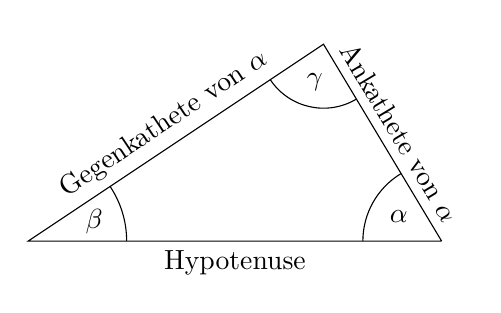
\begin{tikzpicture}[scale=1.25]%,cap=round,>=latex]
					\coordinate (B) at (-2cm,-1.cm);
					\coordinate (A) at (2.2cm,-1.0cm);
					\coordinate (C) at (1cm,1.0cm);
					\draw (A) -- node[below] {Hypotenuse} (B) -- node[sloped,above] {Gegenkathete von $\alpha$} (C) -- node[sloped,above] {Ankathete von $\alpha$} (A);
					\tikzset{/tkzmkangle/mark=none}
					\tkzMarkAngle[size=0.65cm](B,C,A)
					\tkzLabelAngle[pos = 0.4](B,C,A){$\gamma$}
					
					\tkzMarkAngle[size=0.8cm](C,A,B)
					\tkzLabelAngle[pos = 0.5](C,A,B){$\alpha$}
					
					\tkzMarkAngle[size=1cm](A,B,C)
					\tkzLabelAngle[pos = 0.7](A,B,C){$\beta$}
				\end{tikzpicture}
			\end{center}
			\begin{tcolorbox}[boxsep=0pt,top=1cm,left=1cm,right=1cm, bottom=.75cm,arc=0pt,auto outer arc,colback=white,colframe=black, enlarge top by=.25cm, enlarge bottom by=.25cm]
				\subsubsection{Kathetensatz}
				Im rechtwinkligen Dreieck ist das Quadrat über einer Kathete flächengleich zu dem Rechteck aus der Hypotenuse und dem der Kathete anliegenden Hypotenusenabschnitt.
				\begin{flalign*}
				b^2=p\cdot c\\
				a^2=q\cdot c&&
				\end{flalign*}
			\end{tcolorbox}
			\begin{tcolorbox}[boxsep=0pt,top=1cm,left=1cm,right=1cm, bottom=.75cm,arc=0pt,auto outer arc,colback=white,colframe=black, enlarge top by=.25cm, enlarge bottom by=.25cm]
				\subsubsection{Höhensatz}
				Im rechtwinkligen Dreieck ist das Quadrat über der Höhe flächengleich zu dem Rechteck aus den beiden Hypotenusenabschnitten.
				\begin{flalign*}
				h^2=p\cdot q&&
				\end{flalign*}
			\end{tcolorbox}
				\begin{tcolorbox}[boxsep=0pt,top=1cm,left=1cm,right=1cm, bottom=.75cm,arc=0pt,auto outer arc,colback=white,colframe=black, enlarge top by=.25cm, enlarge bottom by=.25cm]
				\subsubsection{Sinus, Kosinus und Tangens}
				Sinus, Kosinus und Tangens ordnen einem Winkel im rechtwinkligen Dreieck die Längenverhältnisse der Katheten und Hypotenuse zu.\newline
				\begin{flalign*}
				&\sin(\alpha)=\frac{a}{c}=\frac{Gegenkathete\;von\;\alpha}{Hypotenuse}\\\\
				&\cos(\alpha)=\frac{b}{c}=\frac{Ankathete\;von\;\alpha}{Hypothenuse}\\\\
				&\tan(\alpha)=\frac{a}{b}=\frac{Gegenkathete\;von\;\alpha}{Ankathete\;von\;\alpha}=\frac{\sin(\alpha)}{\cos(\alpha)}\\\\
				&\sin(90°-\alpha)=\cos(\alpha)\\\\
				&\cos(90°-\alpha)=\sin(\alpha)\\\\
				&(\sin(\alpha))^2+(\cos(\alpha))^2=1&&
				\end{flalign*}
			\end{tcolorbox}
		\subsection{Rechnen mit Flächen (Formeln)}
			\begin{tcolorbox}[boxsep=0pt,top=1cm,left=1cm,right=1cm, bottom=.75cm,arc=0pt,auto outer arc,colback=white,colframe=black, enlarge top by=.25cm, enlarge bottom by=.25cm]
				\subsubsection{Dreieck}
				Für ein Dreieck mit der Grundseite $c$ und der Höhe $h_c$ gilt:
				\begin{flalign*}
				&F=\frac{1}{2}\cdot c \cdot h_c&&
				\end{flalign*}
			\end{tcolorbox}
			\begin{tcolorbox}[boxsep=0pt,top=1cm,left=1cm,right=1cm, bottom=.75cm,arc=0pt,auto outer arc,colback=white,colframe=black, enlarge top by=.25cm, enlarge bottom by=.25cm]
				\subsubsection{Kreis}
				Für einen Kreis mit dem Radius $r$, dem Umfang $U$ und der Fläche $F$ gilt:
				\begin{flalign*}
				&U=2\pi r\\\\
				&F=\pi r^2&&
				\end{flalign*}
				Für einen Kreissektor mit dem Radius $r$, der Bogenlänge $b$, der Fläche $F$ und dem Winkel $\alpha$ gilt:
				\begin{flalign*}
				&F=\frac{br}{2}&&
				\end{flalign*}
				Für ein Kreissegment mit dem Radius $r$, der Bogenlänge $b$, der Fläche $F$ und dem Winkel $\alpha$ gilt:
				\begin{flalign*}
				&F=\frac{br}{2}-\frac{1}{2}r^2\cdot \sin(\alpha)&&
				\end{flalign*}
			\end{tcolorbox}
		\subsection{Rechnen mit Körpern (Formeln)}
		\begin{tcolorbox}[boxsep=0pt,top=1cm,left=1cm,right=1cm, bottom=.75cm,arc=0pt,auto outer arc,colback=white,colframe=black, enlarge top by=.25cm, enlarge bottom by=.25cm]
			\subsubsection{Prisma}
			Für ein Prisma mit der Mantelfläche $M$, der Grundfläche $A$, dem Grundflächenumfang $U$, der Oberfläche $O$, dem Volumen $V$ und der Höhe $h$ gilt:
			\begin{flalign*}
			&V=A\cdot h\\\\
			&M=U\cdot h\\\\
			&O=2\cdot A+M&&
			\end{flalign*}
		\end{tcolorbox}
		\begin{tcolorbox}[boxsep=0pt,top=1cm,left=1cm,right=1cm, bottom=.75cm,arc=0pt,auto outer arc,colback=white,colframe=black, enlarge top by=.25cm, enlarge bottom by=.25cm]
			\subsubsection{Pyramide}
			Für eine Pyramide mit der Mantelfläche $M$, der Grundfläche $A$, der Oberfläche $O$, dem Volumen $V$ und der Höhe $h$ gilt:
			\begin{flalign*}
			&V=\frac{1}{3}\cdot A \cdot h\\\\
			&O=2\cdot A+M&&
			\end{flalign*}
		\end{tcolorbox}
		\begin{tcolorbox}[boxsep=0pt,top=1cm,left=1cm,right=1cm, bottom=.75cm,arc=0pt,auto outer arc,colback=white,colframe=black, enlarge top by=.25cm, enlarge bottom by=.25cm]
			\subsubsection{Zylinder}
			Für einen Zylinder mit der Grundfläche $A$, dem Radius der Grundfläche $r$, der Oberfläche $O$, dem Volumen $V$ und der Höhe $h$ gilt:
			\begin{flalign*}
			V=\pi \cdot r^2\cdot h&&
			\end{flalign*}
			Für einen geraden Zylinder gilt außerdem:
			\begin{flalign*}
				O=2\pi r\cdot (r+h)&&
			\end{flalign*}
		\end{tcolorbox}		
		\begin{tcolorbox}[boxsep=0pt,top=1cm,left=1cm,right=1cm, bottom=.75cm,arc=0pt,auto outer arc,colback=white,colframe=black, enlarge top by=.25cm, enlarge bottom by=.25cm]
			\subsubsection{Kegel}
			Für einen Kegel mit der Grundfläche $A$, dem Radius der Grundfläche $r$, der Oberfläche $O$, dem Volumen $V$, dem Abstand der Spitze zu einem Punkt der Kreislinie $s$ und der Höhe $h$ gilt:
			\begin{flalign*}
			V=\frac{1}{3}\pi\cdot r^2 \cdot h&&
			\end{flalign*}
			Für einen geraden Kegel gilt außerdem:
			\begin{flalign*}
			&s=\sqrt{h^2+r^2}\\\\
			&O=\pi r \cdot (r+s)&&
			\end{flalign*}
		\end{tcolorbox}
	\section{Funktionen}
		\subsection{Allgemeines}
				\begin{tcolorbox}[boxsep=0pt,top=1cm,left=1cm,right=1cm, bottom=.75cm,arc=0pt,auto outer arc,colback=white,colframe=black, enlarge top by=.25cm, enlarge bottom by=.25cm]
					\subsubsection{Monotonie}
						Seien $x_1$ und $x_2$ zwei Argumente einer Funktion, so gelten folgende Definitionen:\newline\newline
						\textbf{Monoton wachsend}
						\begin{flalign*}
						wenn\;x_1\le x_2\; und\; f(x_1)\le f(x_2)&&
						\end{flalign*}
						\textbf{Streng monoton wachsend}
						\begin{flalign*}
						wenn\;x_1< x_2\; und\; f(x_1)< f(x_2)&&
						\end{flalign*}
						\textbf{Monoton fallend}
						\begin{flalign*}
						wenn\;x_1\le x_2\; und\; f(x_1)\ge f(x_2)&&
						\end{flalign*}
						\textbf{Streng monoton fallend}
						\begin{flalign*}
						wenn\;x_1< x_2\; und\; f(x_1)> f(x_2)&&
						\end{flalign*}
				\end{tcolorbox}
				\begin{tcolorbox}[boxsep=0pt,top=1cm,left=1cm,right=1cm, bottom=.75cm,arc=0pt,auto outer arc,colback=white,colframe=black, enlarge top by=.25cm, enlarge bottom by=.25cm]
					\subsubsection{Besondere Stellen}
					Für manche Stelle einer Funktion werden besondere Begriffe benutzt. Hinweis: $D_f$ ist der Definitionsbereich der Funktion und $I$ ein beliebig kleiner offener Intervall, der $x_{max}$ bzw. $x_{min}$ beinhaltet.\newline\newline
					\textbf{Globale Maximalstelle}
					\begin{flalign*}
						wenn\;f(x_{max})\ge f(x)\; aller\;x\in D_f&&
					\end{flalign*}
					\textbf{Lokale Maximalstelle}
					\begin{flalign*}
						wenn\;f(x_{max})\ge f(x)\; aller\;x\in D_f\cap I&&
					\end{flalign*}
					\textbf{Globale Minimalstelle}
					\begin{flalign*}
						wenn\;f(x_{max})\le f(x)\; aller\;x\in D_f&&
					\end{flalign*}
					\textbf{Lokale Minimalstelle}
					\begin{flalign*}
						wenn\;f(x_{max})\le f(x)\; aller\;x\in D_f\cap I&&
					\end{flalign*}
					Maximal- und Minimalstellen werden auch als Extremalstellen bezeichnet.\newline\newline
					\textbf{Gerade}
					\begin{flalign*}
						wenn\;f(-x)=f(x)&&
					\end{flalign*}
					\textbf{Ungerade}
					\begin{flalign*}
						wenn\;f(-x)=-f(x)&&
					\end{flalign*}
					Achtung: Eine Funktion kann nur gerade oder ungerade sein, wenn ihr Definitionsbereich symmetrisch zum Nullpunkt auf $x$-Achse ist.
				\end{tcolorbox}
		\subsection{Potenz- und Wurzelfunktionen}
			\begin{tcolorbox}[boxsep=0pt,top=1cm,left=1cm,right=1cm, bottom=.85cm,arc=0pt,auto outer arc,colback=white,colframe=black, enlarge top by=.25cm, enlarge bottom by=.25cm]
				Potenzfunktionen in der Form $f(x)=x^m$ mit $m\in\mathbb{N}_0$ und $D_f=\mathbb{R}$ heißen \textbf{Monome} (im Gegensatz zu Polynomen). Potenzfunktionen mit der Form $x^{\frac{m}{n}}$ sind \textbf{Wurzelfunktionen}, wenn $n\ge 2$ gilt und der Bruch keine ganze Zahl ist. An der Potenz kann man erkennen, ob eine Funktion gerade ($x^{2n}$) oder ungerade ($x^{2n-1}$) ist. Hier sind einige Beispiele für Graphen von Wurzelfunktionen:\newline
				\makeplot{{x^3},{x^2},{x^(3/2)},{x^(2/3)},{x^(-1/2)},{x^(-2)},{x^(-3)}}{{$f(x)=x^3$},{$f(x)=x^2$},{$f(x)=x^{\frac{3}{2}}$},{$f(x)=x^{\frac{2}{3}}$},{$f(x)=x^{-\frac{1}{2}}$},{$f(x)=x^{-2}$},{$f(x)=x^{-3}$}}{{1,-1},{1,-2},{4,-1},{4,-2},{7,-1},{7,-2},{10,-1}}{-6,6}{-6,6}{-10:10}{300}{14cm,7cm}
			\end{tcolorbox}
			\subsubsection{Wurzelgleichungen}
			Bei Wurzelgleichungen wird zuerst der Definitionsbereich bestimmt werden, also die Menge an reellen Zahlen, für die der Radikand positiv oder gleich Null ist. Zur Lösung von Wurzelgleichungen wird die Wurzel auf einer Seite der Gleichung isoliert. Dann werden beide Seiten der Gleichung mit dem Wurzelexponenten (im Falle der Quadratwurzel also mit 2) so lange potenziert, bis alle Wurzeln eliminiert sind. Man bekommt also unter Umständen durch das Quadrieren (das Potenzieren mit einer geraden Zahl ist keine Äquivalenzumformung) neue Lösungen (Scheinlösungen) hinzu, die die ursprüngliche Gleichung nicht hatte. Die Probe ist folglich für Wurzelgleichungen unverzichtbar!\newline\newline
			Beispiel ($\sqrt{2x+1}=x-17$):
			\begin{flalign*}
			2x+1&\ge 0\\
			x&\ge -\frac{1}{2}&&
			\end{flalign*}
			Damit haben wir den Definitionsbereich. Jetzt kann man nach der Lösung suchen.
			\begin{flalign*}
			\sqrt{2x+1}&=x-17\\
			2x+1&=(x-17)^2\\
			2x+1&=x^2-34x+289\\
			x^2-36x+288&=0\\
			x_1&=12\\
			x_2&=24&&
			\end{flalign*}
			Jetzt MUSS man das Ergebnis noch überprüfen, indem man die Werte $x_1$ und $x_2$ in die ursprüngliche Gleichung einsetzt.
			\begin{flalign*}
			\sqrt{2x_1+1}&=x_1-17\\
			\sqrt{2\cdot 12+1}&=12-17\\
			\sqrt{25}&=-5\\
			5&=-5&&
			\end{flalign*}
			Das Einsetzen von $x_1$ liefert keine wahre Aussage und ist somit nicht Teil der Lösungsmenge.
			\begin{flalign*}
			\sqrt{2x_2+1}&=x_2-17\\
			\sqrt{2\cdot 24+1}&=24-17\\
			\sqrt{49}&=7\\
			7&=7&&
			\end{flalign*}
			Da $x_2$ im Definitionsbereich liegt und beim Einsetzen eine wahre Aussage ergibt, ist es in der Lösungsmenge enthalten.
			\begin{flalign*}
			\mathbb{L}=\{24\}&&
			\end{flalign*}
			Übrigens: Wenn man mehrere Wurzeln in der Gleichung hat, muss man den Definitionsbereich für den Radikanden jeder Wurzel bestimmen.
			\makeplot{{sqrt(abs(2*x+1))},{x-17}}{{$f(x)=\sqrt{2x+1}$},{$f(x)=x-17$}}{{6.5,3.6},{8.3,1.4}}{0,30}{0,10}{-60:60}{600}{17cm,7cm}
			Mithilfe dieser Grafik kann man das Ergebnis wunderbar visualisieren, denn das Ergebnis ist der $x$-Wert des Schnittpunkts der beiden Funktionen, die man aus der linken und rechten Seite der Wurzelgleichung entnehmen kann.
			\subsubsection{Wurzelgleichungen mit mehreren Wurzeln (Beispiel)}
			\begin{flalign*}
			\sqrt{8x-14}+\sqrt{5x-2}&=\sqrt{27x-36}\\
			(\sqrt{8x-14}+\sqrt{5x-2})^2&=27x-36\\
			8x-14+2\sqrt{(8x-14)(5x-2)}+5x-2&=27x-36\\
			2\sqrt{(8x-14)(5x-2)}&=14x-20\\
			\sqrt{(8x-14)(5x-2)}&=7x-10\\
			40x^2-86x+28&=(7x-10)^2\\
			40x^2-86x+28&=49x^2-140x+100\\
			0&=9x^2-54x+72\\
			0&=x^2-6x+8&&
			\end{flalign*}
			Jetzt kann man die \highlight{subsubsec:pqformel}{p-q-Formel} anwenden und erhält die Lösungsmenge $\mathbb{L}=\{2;4\}$.
		\subsection{Betragsfunktionen}
			\label{subsec:betragsfunktionen}
			Um mit Betragsgleichungen oder auch Betragsfunktionen rechnen zu können muss man mehrere Fälle betrachten. Nämlich einmal den Fall, dass im Betrag ein Wert größer oder gleich $0$ entsteht und einmal den Fall, dass das Ergebnis im Betrag kleiner als Null ist. Betrachten wir einmal ein Beispiel, wo man den Schnittpunkt zwischen $f(x)=\vert x+1\vert$ und $f(x)=x+2$ finden soll.\newline
			\makeplot{{x+2},{abs(x+1)}}{{$f(x)=x+2$},{$f(x)=\vert x+1\vert$}}{{5.5,4},{9.5,3.2}}{-5,5}{-4,4}{-10:10}{100}{17cm,7cm}
			Zunächst setzen wir unsere Funktionen gleich und erhalten eine Betragsgleichung. Dann betrachten wir die verschiedenen Fälle für den Betrag.
			\begin{flalign*}
			\vert x+1\vert &= \left\{x+1\;\;\;\;\;\;\;\;\;Fall\;x\ge -1  \atop -(x+1)\;\;\;\;Fall\;x<-1 \right.&&
			\end{flalign*}
			Durch die Fallunterscheidung kann man die Betragsstriche weglassen, indem man jeden Fall einzeln betrachtet. Hinterher muss man aber noch überprüfen, ob das Ergebnis der Bedingung für $x$ in dem Fall entspricht.\newline\newline
			Fall $x\ge-1$ ($x+1$ ist positiv):
			\begin{flalign*}
			x+1&=x+2 &\mid-x &&&&&&&&&&\\
			1&=2&&
			\end{flalign*}
			Für den Fall $x\ge-1$ gibt es keine Lösung, also weiter zum nächsten Fall.\newline\newline
			Fall $x<-1$ ($x+1$ ist negativ):
			\begin{flalign*}
			-x-1&=x+2 &\mid+x-2 &&&&&&&&&&\\
			2x&=-3\\
			x&=-\frac{3}{2}&&
			\end{flalign*}
			Damit haben wir unsere Lösungsmenge, denn wir bekommen für den Fall $-(x<-1)$ ein Ergebnis, welches dem Kriterium $x<-1$ entspricht.
			\begin{flalign*}
			\mathbb{L}=\left\{-\frac{3}{2}\right\}&&
			\end{flalign*}
			Durch einsetzen dieser $x$-Koordinate, finden wir auch den dazugehörigen $y$-Wert: $P\left(-\frac{3}{2}\mid\frac{1}{2}\right)$:
			\subsubsection{Betragsgleichungen mit mehreren Beträgen}
			Haben wir mehrere Beträge in unserer Gleichung, haben wir auch mehrere Fälle zu betrachten. Schon wir uns das an einem Beispiel an, indem wir die Schnittpunkte von $f(x)=\vert x+1 \vert + 5$ und $f(x)=\vert 2x-4 \vert$ suchen.
			\makeplot{{abs(x+1)+5},{abs(2*x-4)}}{{$f(x)=\vert x+1 \vert + 5$},{$f(x)=\vert 2x-4 \vert$}}{{6.9,3.6},{10,1.7}}{-4,14}{0,20}{0:20}{300}{17cm,7cm}
			Zunächst setzen wir die Funktionen wieder gleich.
			\begin{flalign*}
			\vert x+1 \vert + 5=\vert 2x-4 \vert&&
			\end{flalign*}
			Die Fälle müssen wir alle einzeln betrachten. Das heißt, wir haben insgesamt 4 Fälle. Wir schauen uns zunächst die beiden Fälle eines Betrages an und dann innerhalb dieser Fälle betrachten wir die Fälle für den zweiten Betrag.\newline\newline
			1. Fall für $\vert x+1 \vert$: $x\ge-1$ ($x+1$ ist positiv)
			\begin{flalign*}
			x+1+5&=\vert 2x-4\vert\\
			x+6&=\vert 2x-4\vert&&
			\end{flalign*}
			Innerhalb dieses ersten Falles unterscheiden wir jetzt noch einmal für den übrigen Betrag.
			\begin{tcolorbox}[boxsep=0pt, left=2em, top=1em, bottom=1em,right=0cm,arc=0pt,auto outer arc,colback=white,colframe=white]
				1. Fall für $\vert2x-4\vert$: $x\ge2$ ($2x-4$ ist positiv)
				\begin{flalign*}
				x+6&=2x-4\\
				x+10&=2x\\
				10&=x&&
				\end{flalign*}
				Jetzt müssen wir überprüfen, ob $x\ge2$ und $x\ge-1$ für $x=10$ gelten. Das ist der Fall daher haben wir schon mal einen Teil unserer Lösungsmenge. Auf der Grafik kann man auch sehen, dass sich die beiden Graphen dort schneiden.\newline\newline
				2. Fall für $\vert2x-4\vert$: $x<2$ ($2x-4$ ist negativ)
				\begin{flalign*}
				x+6&=-(2x-4)\\
				x+6&=-2x+4\\
				3x+6&=4\\
				3x&=-2\\
				x&=-\frac{2}{3}&&
				\end{flalign*}
				Wir überprüfen jetzt wieder, ob $x<2$ und $x\ge-1$ für $x=-\frac{2}{3}$ gelten. Da das der Fall ist, können wir auch dieses $x$ zu unserer Lösungsmenge hinzufügen.
			\end{tcolorbox}
			\noindent 2. Fall für $\vert x+1 \vert$: $x<-1$ ($x+1$ ist negativ)
			\begin{flalign*}
			-(x+1)+5&=\vert 2x-4\vert\\
			-x+4&=\vert 2x-4\vert&&
			\end{flalign*}
			\begin{tcolorbox}[boxsep=0pt, left=2em, top=1em, bottom=1em,right=0cm,arc=0pt,auto outer arc,colback=white,colframe=white]
				1. Fall für $\vert2x-4\vert$: $x\ge2$ ($2x-4$ ist positiv)\newline\newline
				In diesem Fall müssen wir gar nicht erst versuchen $x$ auszurechnen, denn es gibt keine Zahl, die sowohl $x\ge2$, als auch $x<-1$ erfüllt.\newline\newline
				2. Fall für $\vert2x-4\vert$: $x<2$ ($2x-4$ ist negativ)
				\begin{flalign*}
				-x+4&=-(2x-4)\\
				-x+4&=-2x+4\\
				-x&=-2x\\
				x&=0&&
				\end{flalign*}
				Wir haben jetzt $x=0$ als Lösung, jedoch erfüllt dieses Ergebnis nicht die Bedingung $x<-1$ und ist daher auch nicht in der Lösungsmenge enthalten.
			\end{tcolorbox}
			\noindent Abschließend können wir feststellen, dass unsere Lösungsmenge $\mathbb{L}=\left\{10;-\frac{2}{3}\right\}$ ist. Durch Einsetzen in eine der beiden Funktionen erhalten wir dann unsere Schnittpunkte $P_1(10\mid 16)$ und $P_2\left(-\frac{2}{3}\mid\frac{16}{3}\right)$.
		\subsection{Polynomfunktionen}
			\begin{tcolorbox}[boxsep=0pt,top=1cm,left=1cm,right=1cm, bottom=.85cm,arc=0pt,auto outer arc,colback=white,colframe=black, enlarge top by=.25cm, enlarge bottom by=.25cm]
				Polynome sind die Summe aus den Vielfachen von Monomen. Eine Polynomfunktion mit den Koeffizienten $a_n$ hat folgende Form:
				\begin{flalign*}
				p(x)=a_nx^n+a_{n-1}x^{n-1}+...+a_1x^1+1_0&&
				\end{flalign*}
				Das Verhalten einer Polynomfunktion hängt für $x\to \infty$ vom Summanden mit der höchsten Potenz und für $x\to 0$ vom Summanden mit der niedrigsten Potenz ab. Für die Symmetrie der Funktion gilt weiterhin, dass bei geraden Potenzen eine gerade Funktion vorliegt und bei ungeraden Potenzen eine ungerade Funktion. Hat ein Polynom jedoch sowohl gerade, wie auch ungerade Exponenten, so kann man beides ausschließen.\newline\newline
				\textbf{Nullstellen}\newline\newline
				Polynome n-ten Grades haben maximal n Nullstellen.
				\begin{flalign*}
					p(x)=a_{2k-1}x^{2k-1}+...+a_1x+a_0,\;wenn\;a_{2k-1}\neq 0&&
				\end{flalign*}
				Polynome ungeraden Grades haben mindestens eine Nullstelle.
				\begin{flalign*}
					p(x)=a_{2k}x^{2k}+...+a_2x^2+a_0,\;wenn\;a_{2k}\ge 0\;und\;a_0>0&&
				\end{flalign*}
				Polynome geraden Grades besitzen keine Nullstellen.\newline
				\makeplot{{x^4-x^3-2*x^2},{x^4},{-2*x^2}}{{$f(x)=x^4-x^3-2x^2$},{$f(x)=x^4$},{$f(x)=-2x^2$}}{{5,3.2},{5.7,5},{5.9,1}}{-7,3}{-4,4}{-10:10}{400}{14cm,7cm}
			\end{tcolorbox}
	
		\subsubsection{Lösen durch Substitution}
		In diesem Beispiel werden die Nullstellen der Funktion mithilfe von \highlight{subsec:substitution}{Substitution} und anschließendem Anwenden der \highlight{subsubsec:pqformel}{p-q-Formel} ermittelt.\newline
		\makeplot{{x^4-5*x^2+2}}{{$p(x)=x^4-5x^2+2$}}{{12.5,1.3}}{-6,6}{-6,6}{-30:60}{300}{17cm,7cm}
		\begin{flalign*}
			p(x)&=x^4-5x^2+2\\
			0&=x^4-5x^2+2\\
			0&=u^2-5u+2\\
			u_{1,2}&=\frac{5}{2}\pm\sqrt{\left(-\frac{5}{2}\right)^2-2}\\
			u_1&=\frac{5+\sqrt{17}}{2}\\
			u_2&=\frac{5-\sqrt{17}}{2}\\\\
			x_{1,2}^2&=\frac{5+\sqrt{17}}{2}\\
			x_{1,2}^2&=\pm 2,135779205\\\\
			x_{3,4}^2&=\frac{5-\sqrt{17}}{2}\\
			x_{3,4}^2&=0,6621534469\\\\
			\mathbb{L}&=\{-2,135779205;-0,6621534469;0,6621534469;2,135779205\}&&
		\end{flalign*}
		\hrulefill
		\subsubsection{Lösen durch Faktorisierung}
		In diesem Beispiel werden die Nullstellen der Funktion mithilfe von \highlight{subsubsec:ausklammern}{Faktorisierung durch Ausklammern} ermittelt.\newline
		\makeplot{{x^5-3*x^3}}{{$p(x)=x^5-3x^3$}}{{11.75,1.3}}{-6,6}{-6,6}{-30:60}{300}{17cm,7cm}
		\begin{flalign*}
		p(x)&=x^5-3x^3\\
		0&=x^5-3x^3\\
		0&=x^2(x^2-3)\\
		0&=x^2(x^2-\sqrt{3})(x^2+\sqrt{3})\\
		\mathbb{L}&=\{-\sqrt{3};0;\sqrt{3}\}&&
		\end{flalign*}
		\hrulefill
		\subsubsection{Lösen mit binomischen Formeln}
		In diesem Beispiel wird Funktion mithilfe der \highlight{sec:binomischeformeln}{binomischen Formeln} so vereinfacht, dass man die Nullstellen ganz einfach ablesen kann.\newline
		\makeplot{{x^4-2*x^2+1}}{{$p(x)=x^4-2x^2+1$}}{{11.6,3.2}}{-6,6}{-6,6}{-30:60}{300}{17cm,7cm}
		\begin{flalign*}
		p(x)&=x^4-4x^2+1\\
		0&=x^4-4x^2+1\\
		0&=(x^2-1)^2\\
		x&=\pm 1\\
		\mathbb{L}&=\{-1;1\}&&
		\end{flalign*}
		\hrulefill
		\subsubsection{Lösen durch Polynomdivision}
			Wenn alle anderen Stränge reißen, ist man leider gezwungen die Polynomdivision durchzuführen. Um damit beginnen zu können, braucht man aber mindestens eine Nullstelle, die man durch Raten findet. Für das Beispiel unten finden wir so heraus, dass eine Nullstelle $x_1=1$ ist. Jetzt stellen wir $x=1$ nach $0$ um und erhalten $0=x-1$. Anschließend teilen wir unser Polynom durch $x-1$.\newline
			\makeplot{{2*x^3-5*x^2-2*x+5}}{{$p(x)=2x^3-5x^2-2x+5$}}{{3.9,3.2}}{-6,6}{-6,6}{-30:60}{300}{17cm,7cm}
			\begin{flalign*}
			(2x^3-5x^2-2x+5):(x-1)&&
			\end{flalign*}
			Zunächst teilt man den Term mit der höchsten Potenz $2x^3$ durch $x$ und erhält $2x^2$. Das ist der erste Teil unseres Ergebnisses.
			\begin{flalign*}
			(2x^3-5x^2-2x+5):(x-1)=2x^2...&&
			\end{flalign*}
			Jetzt muss man zurück multiplizieren, indem man den Term $2x^2$, den wir gerade bekommen haben, mit unserem ursprünglichen Divisor $x-1$ multiplizieren. Das Ergebnis ziehen wir von unserem Polynom ab und holen anschließend den nächsten Ausdruck runter. Diesen Prozess wiederholen wir jetzt so oft, wie möglich.\newline\newline
			\polylongdiv[style=C,div=:]{2x^3-5x^2-2x+5}{x-1}\newline\newline
			Mit der Funktion, die wir jetzt haben, können wir ganz einfach die restlichen Nullstellen errechnen.\newline
			\makeplot{{2*x^2-3*x-5}}{{$f(x)=2x^2-3x-5$}}{{3.9,3.2}}{-6,6}{-10,10}{-30:60}{300}{17cm,7cm}
			\begin{flalign*}
				f(x)&=2x^2-3x-5\\
				0&=2x^2-3x-5\\
				0&=x^2-1,5x-2,5\\
				x_{1,2}&=\frac{1,5}{2}\pm\sqrt{\left(-\frac{1,5}{2}\right)^2+2,5}\\
				x_1&=2,5\\
				x_2&=-1\\
				\mathbb{L}&=\{-1;1;2,5\}&&
			\end{flalign*}
		\subsection{Exponentialfunktionen}
			\begin{tcolorbox}[boxsep=0pt,top=.75cm,left=1cm,right=1cm, bottom=.75cm,arc=0pt,auto outer arc,colback=white,colframe=black, enlarge top by=.25cm, enlarge bottom by=.25cm]
				Eine Funktion der Form $f(x)=a^x$ wird als Exponentialfunktion bezeichnet, denn die Variable $x$ steht im Exponenten. Speziell wird die Funktion $f(x)=e^x$ als \textit{natürliche Exponentialfunktion} bezeichnet.
				\makeplot{{e^x},{e^(-x)}}{{$f(x)=e^x$},{$f(x)=e^{-x}$}}{{8,3.3},{4.1,3.3}}{-6,6}{-6,6}{-10:10}{300}{14cm,7cm}
			\end{tcolorbox}
			\subsubsection{Lösen von Exponentialgleichungen}
				Zum Lösen von Exponentialgleichungen brauchen wir in der Regel den \highlight{subsec:logarithmusgesetze}{Logarithmus}. Wie das funktioniert, sehen wir an dem Beispiel hier drunter. Dabei ist die Nullstelle der Funktion zu bestimmen. In diesem Beispiel sollte man sich außerdem nochmal daran erinnern, dass $\sqrt[n]{x}$ dasselbe ist, wie $x^{\frac{1}{n}}$.
				\makeplot{{(7^x)^(1/4)-4}}{{$f(x)=\sqrt[4]{7^x}-4$}}{{10,3.2}}{-6,6}{-10,10}{-30:30}{300}{17cm,7cm}
				\begin{flalign*}
					f(x)&=\sqrt[4]{7^x}-4\\
					0&=\sqrt[4]{7^x}-4 && \mid +4 &&&&&&&&&&&&& \\
					4&=7^{\frac{x}{4}} && \mid log_7() &&&&&&&&&&&&& \\
					0,7124143742&=\frac{x}{4} && \mid \cdot 4 &&&&&&&&&&&&& \\
					x&=2,849657497\\
					\mathbb{L}=\{2,849657497\}&&
				\end{flalign*}
		\subsection{Logarithmusfunktionen}
			\begin{tcolorbox}[boxsep=0pt,top=.75cm,left=1cm,right=1cm, bottom=.75cm,arc=0pt,auto outer arc,colback=white,colframe=black, enlarge top by=.25cm, enlarge bottom by=.25cm]
				Funktionen wie $f(x)=log_3(x^2)$ werden als Logarithmusfunktionen bezeichnet, da sie einen oder mehrere Logarithmen beinhalten. Speziell bezeichnet man $f(x)=ln(x)$ als \textit{natürliche Logarithmusfunktion} und $f(x)=lg(x)$ als \textit{dekadische Logarithmusfunktion}.
				\makeplot{{ln(x)},{log10(x)},{-ln(abs(x))}, {log2(x)}}{{$f(x)=ln(x)$},{$f(x)=lg(x)$},{$f(x)=-ln(\vert x\vert)$},{$f(x)=log_2(x)$}}{{8,4.3},{11,4.8},{2,1},{8,1}}{-6,6}{-4,4}{-200:200}{500}{14cm,7cm}
			\end{tcolorbox}
			\subsubsection{Lösen von Logarithmusgleichungen}
				Gesucht wird hier die Nullstelle einer Logarithmusfunktion gesucht. Hinweis: Um einen Logarithmus aufzulösen musst du beide Seiten der Gleichung als Exponent zur Basis des jeweiligen Logarithmus setzen. Um dort hinzu kommen hilft es enorm, die Gleichung zunächst umzuformen. Wenn du Schwierigkeiten mit den Umformungen in diesem Beispiel hast, schaue dir noch einmal die \highlight{subsec:potenzgesetze}{Potenzgesetze} und \highlight{subsec:logarithmusgesetze}{Logarithmusgesetze} an.
				\makeplot{{3*log10(x^3)-2*log10(x^2)-4}}{{$f(x)=3\cdot lg(x^3)-2\cdot lg(x^2)-4$}}{{11,3.3}}{-10,10}{-10,10}{-20:20}{300}{17cm,7cm}
				\begin{flalign*}
					f(x)&=3\cdot lg(x^3)-2\cdot lg(x^2)-4\\
					0&=3\cdot lg(x^3)-2\cdot lg(x^2)-4\\
					0&=lg((x^3)^3)-lg((x^2)^2)-4&&\mid +4&&&&&&&&&&&\\
					lg\left(\frac{x^9}{x^4} \right)&=4\\
					lg(x^5)&=4&&\mid 10^{()}\\
					10^{lg(x^5)}&=10^4\\
					x^5&=10^4&&\mid \sqrt[5]{\;}\\
					x&=6,309573445\\
					\mathbb{L}&=\{6,309573445\}&&
				\end{flalign*}
		\subsection{Trigonometrische Funktionen}
			\begin{tcolorbox}[boxsep=0pt,top=.85cm,left=1cm,right=1cm, bottom=.75cm,arc=0pt,auto outer arc,colback=white,colframe=black, enlarge top by=.25cm, enlarge bottom by=.25cm]
				Trigonometrische Funktionen oder auch Winkelfunktionen genannt, beinhalten die aus der \highlight{sec:geometrie}{Geometrie} bekannten winkelabhängigen Funktionen, wie Sinus, Kosinus und Tangens. Dabei sind diese Funktionen hier allerdings abhängig von der Variable $x$ und damit im Bogenmaß, nicht im Gradmaß. Beim Taschenrechner muss man darauf achten, dass der richtige Modus eingestellt ist, ansonsten kann es sein, dass man versehentlich im falschen Maß rechnet. Auf dem CASIO fx-86DE PLUS, drückt man Shift, dann Setup und wählt dort die 3:Deg (engl. degree) für Gradmaß oder 4:Rad (engl. radian) fürs Bogenmaß.
				\makeplot{{sin(deg(x))},{cos(deg(x))},{tan(deg(x))}}{{$f(x)=\sin(x)$},{$f(x)=\cos(x)$},{$f(x)=\tan(x)$}}{{1.5,-1},{4.5,-1},{7.5,-1}}{-10,10}{-2,2}{-10:10}{200}{14cm,7cm}
				Anmerkung: Die Nullstellen des Sinus sind die Extremstellen des Kosinus und umgekehrt. Ebenso habe Sinus und Tanges dieselben Nullstellen.
			\end{tcolorbox}
		\subsection{Verkettete Funktionen}
				\begin{tcolorbox}[boxsep=0pt,top=.85cm,left=1cm,right=1cm, bottom=.75cm,arc=0pt,auto outer arc,colback=white,colframe=black, enlarge top by=.25cm, enlarge bottom by=.25cm]
				Verkettungen sind eigentliche keine eigene Funktionsart, sondern eine Möglichkeit Funktionen durch Zusammensetzung zu transformieren. Man schreibt das als $f\circ g$ ("f nach g"). Man spricht hier bei $g$ auch von der \textit{inneren Funktion}, da sie als Argument in die \textit{äußere Funktion} $f$ eingesetzt wird.
				\makeplot{{sin(deg(x))},{(x^2)/2},{sin(deg((x^2)/2))}}{{$f(x)=\sin(x)$},{$g(x)=\frac{x^2}{3}$},{$f\circ g(x)=\sin(\frac{x^2}{3})$}}{{1.5,-1},{4.5,-1},{8,-1}}{-10,10}{-2,2}{-10:10}{500}{14cm,7cm}
			\end{tcolorbox}
\end{document}